%& C:\Users\gabri\AppData\Roaming\TikzEdt\TikzEdt\021~1.0\TEMP_H~1
\begin{document}
\usetikzlibrary{patterns,arrows,decorations.pathreplacing}

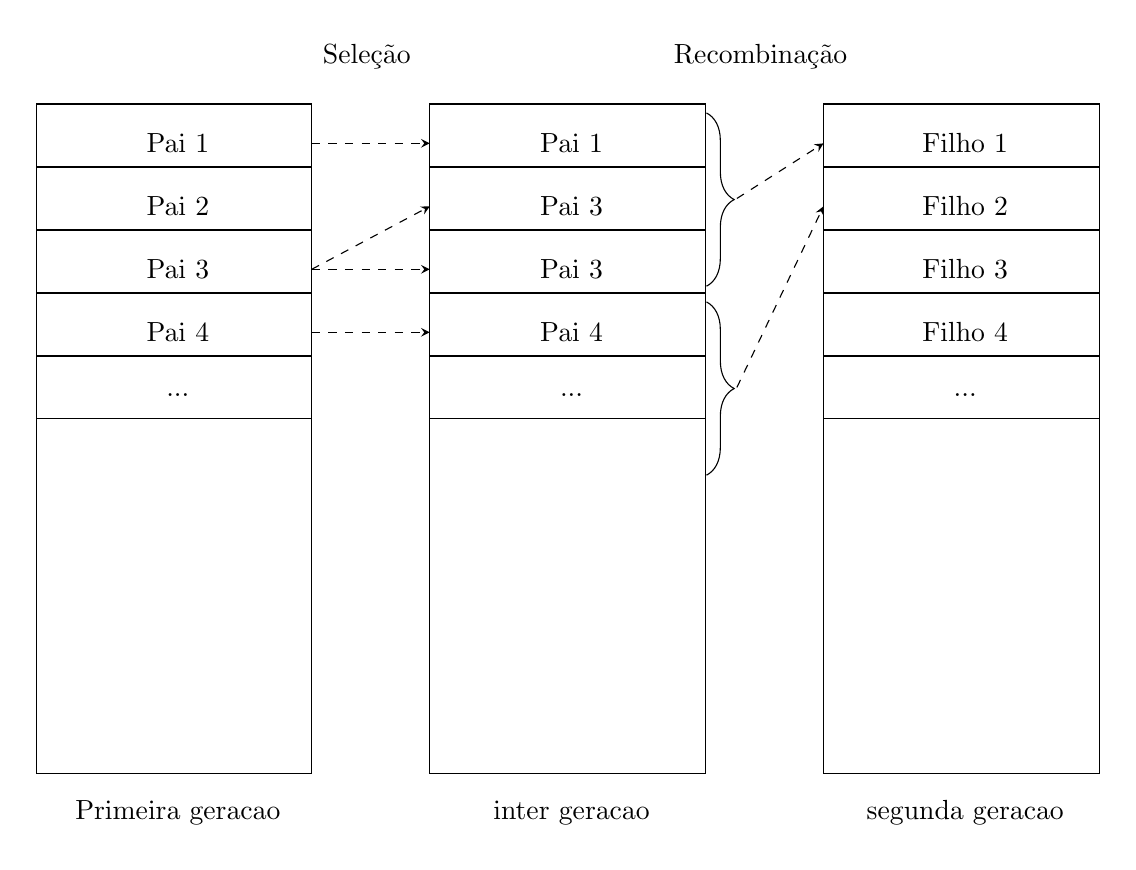
\begin{tikzpicture}
			
\draw  (-5.0,4.0) rectangle (-1.5,-4.5);
\draw  (0.0,4.0) rectangle (3.5,-4.5);
\draw  (5.0,4.0) rectangle (8.5,-4.5);

\draw [] (-5,3.2) -- (-1.5,3.2);
\draw [] (-5,2.4) -- (-1.5,2.4);
\draw [] (-5,1.6) -- (-1.5,1.6);
\draw [] (-5,0.8) -- (-1.5,0.8);
\draw [] (-5,0) -- (-1.5,0);

\node at (-3.2,3.5) {Pai 1};
\node at (-3.2,2.7) {Pai 2};
\node at (-3.2,1.9) {Pai 3};
\node at (-3.2,1.1) {Pai 4};
\node at (-3.2,0.3) {...};

\draw [dashed, -stealth] (-1.5,3.5) -- (0,3.5);
\draw [dashed, -stealth] (-1.5,1.9) -- (0,2.7);
\draw [dashed, -stealth] (-1.5,1.9) -- (0,1.9);
\draw [dashed, -stealth] (-1.5,1.1) -- (0,1.1);

\draw [] (0,3.2) -- (3.5,3.2);
\draw [] (0,2.4) -- (3.5,2.4);
\draw [] (0,1.6) -- (3.5,1.6);
\draw [] (0,0.8) -- (3.5,0.8);
\draw [] (0,0) -- (3.5,0);

\node at (1.8,3.5) {Pai 1};
\node at (1.8,2.7) {Pai 3};
\node at (1.8,1.9) {Pai 3};
\node at (1.8,1.1) {Pai 4};
\node at (1.8,0.3) {...};

\draw [] (5,3.2) -- (8.5,3.2);
\draw [] (5,2.4) -- (8.5,2.4);
\draw [] (5,1.6) -- (8.5,1.6);
\draw [] (5,0.8) -- (8.5,0.8);
\draw [] (5,0) -- (8.5,0);

\node at (6.8,3.5) {Filho 1};
\node at (6.8,2.7) {Filho 2};
\node at (6.8,1.9) {Filho 3};
\node at (6.8,1.1) {Filho 4};
\node at (6.8,0.3) {...};


\node at (-0.8,4.6) {Seleção};
\node at (4.2,4.6) {Recombinação};


\node at (-3.2,-5) {Primeira geracao};
\node at (1.8,-5) {inter geracao};
\node at (6.8,-5) {segunda geracao};

\draw [decorate,decoration={brace,amplitude=10pt},xshift=0.4pt,yshift=-0.4pt](3.5,3.9) -- (3.5,1.7);
\draw [decorate,decoration={brace,amplitude=10pt},xshift=0.4pt,yshift=-0.4pt](3.5,1.5) -- (3.5,-0.7);
\draw [dashed, -stealth] (3.9,2.8) -- (5.0,3.5);
\draw [dashed, -stealth] (3.9,0.4) -- (5.0,2.7);



\usetikzlibrary{calc}
\pgftransformreset
\node[inner sep=0pt,outer sep=0pt,minimum size=0pt,line width=0pt,text width=0pt,text height=0pt] at (current bounding box) {};
%add border to avoid cropping by pdflibnet
\foreach \border in {0.1}
  \useasboundingbox (current bounding box.south west)+(-\border,-\border) rectangle (current bounding box.north east)+(\border,\border);
\newwrite\metadatafile
\immediate\openout\metadatafile=\jobname_BB.txt
\path
  let
    \p1=(current bounding box.south west),
    \p2=(current bounding box.north east)
  in
  node[inner sep=0pt,outer sep=0pt,minimum size=0pt,line width=0pt,text width=0pt,text height=0pt,draw=white] at (current bounding box) {
\immediate\write\metadatafile{\p1,\p2}
};
\immediate\closeout\metadatafile
\end{tikzpicture}

\end{document}


t}
ent}
